% --------------------------------------------------------------------------
% Template for WASPAA-2017 paper; to be used with:
%          waspaa17.sty  - WASPAA 2017 LaTeX style file, and
%          IEEEbib.bst - IEEE bibliography style file.
%
% --------------------------------------------------------------------------

\documentclass{article}
\usepackage{waspaa17,amsmath,graphicx,url,times}
%\usepackage{waspaa17,amssymb,amsmath,graphicx,times,url}
\usepackage{color}
\usepackage{subcaption}
\usepackage{tikz}
\usepackage{tabularx}
\usepackage{booktabs}
\usetikzlibrary{calc,chains,shapes,positioning,patterns}
\usepackage{phaistos}
\usepackage{pgfplots}
\usepackage{cite}
\usepackage{graphicx}
\DeclareMathOperator*{\argmin}{arg\,min}
\def\ninept{\def\baselinestretch{.89}\let\normalsize\small\normalsize}
% Title.
% --------------------
\title{Multi-channel late reverberation power spectral density estimation \\ based on nuclear norm minimization}
\name{Ina Kodrasi, Simon Doclo
\thanks{
This work was supported in part by the Cluster of Excellence 1077 ``Hearing4All'', funded by the German Research Foundation (DFG), and the joint Lower Saxony-Israeli Project ATHENA, funded by the State of Lower Saxony.
}}
\address{
University of Oldenburg, Department of Medical Physics and Acoustics  \\ and Cluster of Excellence Hearing4All, Oldenburg, Germany \\
{\tt \{ina.kodrasi,simon.doclo\}@uni-oldenburg.de}\\
}

\begin{document}
\newlength\figureheight
\newlength\figurewidth
\setlength\figureheight{2.1cm}
\setlength\figurewidth{0.4\textwidth}
\ninept
\maketitle


\begin{abstract} 
  Multi-channel methods for estimating the late reverberation power spectral density (PSD) generally assume that the reverberant PSD matrix can be decomposed as the sum of a rank-$1$ matrix and a scaled diffuse coherence matrix.
  To account for modeling or estimation errors in the estimated reverberant PSD matrix, in this paper we propose to decompose this matrix as the sum of a low rank (not necessarily rank-$1$) matrix and a scaled diffuse coherence matrix.
  Among all pairs of scalars and matrices that yield feasible decompositions, the late reverberation PSD can then be estimated as the scalar associated with the matrix of minimum rank.
  Since rank minimization is an intractable non-convex optimization problem, we propose to use a convex relaxation approach and estimate the late reverberation PSD based on nuclear norm minimization~(NNM).
  Experimental results show the advantages of using the proposed NNM-based late reverberation PSD estimator in a multi-channel Wiener filter for speech dereverberation, significantly outperforming a state-of-the-art maximum likelihood-based PSD estimator and yielding a similar or better performance than a recently proposed eigenvalue decomposition-based PSD estimator. 
\end{abstract}

\begin{keywords}
dereverberation, nuclear norm, convex optimization, MWF, PSD estimation
\end{keywords}

\section{Introduction}
\label{sec:intro}
In hands-free communication applications the recorded microphone signals are often corrupted by early and late reverberation, which arises from the superposition of delayed and attenuated copies of the anechoic speech signal.
While early reverberation may be desirable~\cite{Bradley_JASA_2003}, late reverberation may degrade the perceived quality and hinder the intelligibility of speech~\cite{Warzybok_IWAENC_2014}.
Hence, speech enhancement techniques which effectively suppress the late reverberation are required.
In the last decades many single-channel and multi-channel dereverberation techniques have been proposed~\cite{Naylor_Derev_book}, with multi-channel techniques being generally preferred since they are able to exploit both the spectro-temporal and the spatial characteristics of the received microphone signals.
Many such techniques require an estimate of the late reverberation power spectral density~(PSD), e.g.~\cite{Habets_PhD,OSchwartz_ITASLP_2015,Cauchi_EURASIP_2015}.

The late reverberation PSD can be estimated either using single-channel estimators based on a temporal model of reverberation~\cite{Lebart_ACUSTICA_2001,Habets2009a} or multi-channel estimators based on a (spatial) diffuse sound field model of reverberation~\cite{Braun_EUSIPCO_2013,Kuklasinski_EUSIPCO_2014g,Schwartz_WASPAA_2015,Braun_EURASIP_2015,Schwartz_ICASSP_2016,Kuklasinski_ITASLP_2016,Schwartz_EUSIPCO_2016, Kodrasi_HSCMA_2017, Kodrasi_ICASSP_2017}.
Most multi-channel PSD estimators~\cite{Braun_EUSIPCO_2013,Kuklasinski_EUSIPCO_2014g,Schwartz_WASPAA_2015,Braun_EURASIP_2015,Schwartz_ICASSP_2016,Kuklasinski_ITASLP_2016,Schwartz_EUSIPCO_2016} require an estimate of the relative early transfer functions~(RETFs) of the target signal from the reference microphone to all microphones, which may be difficult to accurately estimate, particularly in highly reverberant and noisy scenarios.
Recently, we proposed a multi-channel late reverberation PSD estimator based on an eigenvalue decomposition (EVD), which does not require such RETF estimates~\cite{Kodrasi_HSCMA_2017,Kodrasi_ICASSP_2017}.
Experimental results in~\cite{Kodrasi_ICASSP_2017} show the advantages of using this EVD-based estimator in a multi-channel Wiener filter~(MWF) for speech dereverberation, outperforming the maximum likelihood (ML)-based estimator in~\cite{Kuklasinski_EUSIPCO_2014g} both when the RETFs are perfectly estimated as well as in the presence of RETF estimation errors. 

The EVD-based estimator in~\cite{Kodrasi_ICASSP_2017} relies on the assumption that the reverberant PSD matrix is equal to the sum of a rank-$1$ matrix (corresponding to the direct and early reverberation speech component) and a diffuse coherence matrix scaled with the late reverberation PSD.
However, since the late reverberation is not truly diffuse and since the reverberant PSD matrix in practice is estimated using a signal realization, the estimated reverberant PSD matrix can deviate from this assumption.
In order to account for this deviation, in this paper we propose to model the reverberant PSD matrix as the sum of a low rank (not necessarily rank-$1$) matrix and a scaled diffuse coherence matrix.
  Among all pairs of scalars and matrices that yield feasible decompositions, the late reverberation PSD can be estimated as the scalar associated with the matrix of minimum rank.
   However, since the rank of a matrix is non-convex and non-convex optimization problems are typically hard (if not impossible) to solve, we propose to estimate the late reverberation PSD based on nuclear norm minimization (NNM)~\cite{Fazel_phd,Candes_ACM_2011, Liu_ITPAMI_2013} instead.
The nuclear norm is a convex relaxation of the rank, and hence, NNM-based optimization problems can be efficiently solved~\cite{Fazel_phd}.
Experimental results for several acoustic systems and configurations illustrate the advantages of using the NNM-based PSD estimator in an MWF for speech dereverberation, yielding a similar or better performance than the ML-based and EVD-based PSD estimators.

\section{Configuration and Notation}
\label{sec:intro}
Consider a reverberant and noisy acoustic system with a single speech source and $M \geq 2$ microphones, as depicted in Fig.~\ref{fig: ac_sys}.
In the short-time Fourier transform (STFT) domain, the $M$-dimensional vector of the microphone signals $\mathbf{y}(k,l) = [Y_1(k,l) \; \ldots \; Y_M(k,l)]^T$ at frequency index $k$ and frame index $l$ is given by
\begin{equation}
  \mathbf{y}(k,l)  = \underbrace{\mathbf{x}_{\rm e}(k,l) + \mathbf{x}_{\rm{r}}(k,l)}_{\mathbf{x}(k,l)} + \mathbf{v}(k,l),
\end{equation} 
with $\mathbf{x}(k,l)$ the speech component, $\mathbf{v}(k,l)$ the noise component, $\mathbf{x}_{\rm e}(k,l)$ the direct and early reverberation speech component, and $\mathbf{x}_{\rm r}(k,l)$ the late reverberation speech component.
%The vectors $\mathbf{x}(k,l)$, $\mathbf{v}(k,l)$, $\mathbf{x}_{\rm e}(k,l)$, and $\mathbf{x}_{\rm r}(k,l)$  are defined similarly as $\mathbf{x}(k,l)$.
For simplicity, in the following we assume that the noise component is equal to zero, i.e., $\mathbf{y}(k,l) = \mathbf{x}(k,l)$.
However, the late reverberation PSD estimator proposed in this paper can also be used in noisy scenarios, cf. Section~\ref{sec: nnm}.
% This corresponds to the assumption that the noise is negligible in comparison to the late reverberation, which can be a realistic assumption in several scenarios.
% % For conciseness the frequency index $k$ is omitted in the remainder of this paper.

The direct and early reverberation speech component $\mathbf{x}_{\rm e}(k,l)$ can be expressed as
\begin{figure}[t!]
    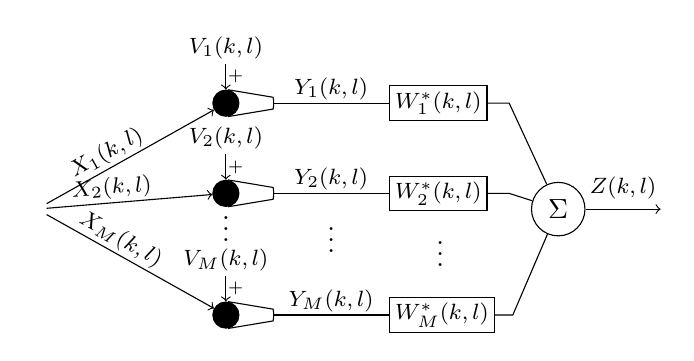
\begin{tikzpicture}
    % Adjustments
    \def\micd{.1cm}                % mic diameter
    \def\micl{.6cm}                % mic length
    \def\micw{.15cm}                % mic width
    \def\micbend{10}               % mic bottom bend
    \def\micdistance{.8cm}         % distance between microphones
    \def\filterdistance{1.9cm}     % distance between microphone and filter
    \def\filteroutline{.9cm}       % length of line which gets out of filter
    \def\sumdistance{1.5cm}        % distance of sum node to the filter
    \def\sumoutline{1cm}           % length of line which gets out of sum
    \def\headdistance{2.4cm}       % distance between microphone and head
%
    % Styles
    \tikzset{%
      mic head/.style={fill=black,draw=black,circle,minimum size=\micd},
      filter/.style={draw,minimum width=1.1cm,inner sep=2pt},
      sum/.style={draw,circle},
      xlabel/.style={inner sep=1pt,above,midway},
      sumlabel/.style={xlabel},
      hlabel/.style={xlabel,sloped,pos=.4},
      head/.style={font=\Large}
    }   %
    % Draw Microphones
    \begin{scope}[start chain=going below,every node/.style={on chain},node distance=\micdistance]
      \node[mic head] (mic1) {};
      \node[mic head] (mic2) {};
      \node[mic head,yshift=-0.5*\micdistance] (mic3) {};
    \end{scope}
    \node[yshift=12pt] at ($(mic2)!.5!(mic3)$) {$\vdots$};
    %
    \foreach \m in {1,2,3} {%
      \coordinate (m1) at ($(mic\m)+(\micl,\micw/2)$);
      \coordinate (m2) at ($(mic\m)+(\micl,-\micw/2)$);
      \draw (tangent cs:node=mic\m,point={(m1)},solution=1) -- (m1) to[bend left=\micbend] (m2) -- (tangent cs:node=mic\m,point={(m2)},solution=2);
    }%
    % Draw Filter
    \foreach \m/\i in {1/1,2/2,3/M} {%
      \node[filter,right=\filterdistance of mic\m] (filter\m) {\footnotesize $W^{*}_{\i}(k,l)$};
      \draw ($(mic\m)+(\micl,0)$) to node[xlabel] (x\m) {\footnotesize $Y_{\i}(k,l)$} (filter\m);
    }
    \node[yshift=3pt] at ($(filter2)!.5!(filter3)$) {$\vdots$};
    \node[yshift=3pt] at ($(x2)!.5!(x3)$) {$\vdots$};
    % Sum Node
    \node[sum] (sum) at ($(filter1)!.5!(filter3)+(\sumdistance,0)$) {$\Sigma$};
    \draw[->] (sum) -- node[above] {\footnotesize $Z(k,l)$} ++(1.3,0);
    % Connect filter with sum
    \foreach \m in {1,2,3} {%
      \draw (filter\m) -- ++(\filteroutline,0) -- (sum);
    }%
    % Head
    \node[head] (head) at ($(mic1)!.5!(mic3)-(\headdistance,0)$) {\PHtattooedHead};
    \node[fill=white,minimum width=4.8pt,minimum height=5.7pt,inner sep=0pt] at ($(head.center)+(2.3pt,-2.5pt)$) {};
    %\node at ($(head.center)+(0.0pt,-20.5pt)$) {\footnotesize $S(k,l)$};
    % Connect head with mics
    \foreach \m/\i in {1/1,2/2,3/M} {%
      \draw[->] (head) -- node[hlabel] {\footnotesize $X_{\i}(k,l)$} (mic\m);
    }
    % Draw noise
    \draw[<-] (mic1) -- node[above=0.1cm] {\footnotesize $V_1(k,l)$} node[right = -0.1cm] {\footnotesize ${}_{+}$} ++(0,0.5);
    \draw[<-] (mic2) -- node[above=0.1cm] {\footnotesize $V_2(k,l)$} node[right = -0.1cm] {\footnotesize ${}_{+}$} ++(0,0.5);
    \draw[<-] (mic3) -- node[above=0.1cm] {\footnotesize $V_M(k,l)$} node[right = -0.1cm] {\footnotesize ${}_{+}$} ++(0,0.5);
  \end{tikzpicture}

  \caption{Acoustic system configuration.}
  \label{fig: ac_sys}
\end{figure} %
\begin{equation}
\label{eq: direct}
\mathbf{x}_{\rm e}(k,l) = S(k,l)\mathbf{d}(k),
\end{equation}
with $S(k,l)$ the target signal (i.e., direct and early reverberation speech component) received by the reference microphone and $\mathbf{d}(k) = [D_1(k) \; \ldots \; D_M(k)]^T$ the vector of RETFs of the target signal from the reference microphone to all microphones.
% The target signal is often defined as the direct component only, such that the vector $\mathbf{d}$ can be computed based on the direction of arrival of the speech source and the geometry of the microphone array~\cite{Braun_EUSIPCO_2013,Kuklasinski_EUSIPCO_2014g,Kuklasinksi_ICASSP_2015,Braun_EURASIP_2015,Schwartz_WASPAA_2015,Schwartz_ICASSP_2016,Kuklasinski_ITASLP_2016,kuklasinski_AES_2016}.
The late reverberation speech component $\mathbf{x}_{\rm r}(k,l)$ is commonly modeled as a diffuse sound component and is assumed to be uncorrelated with the direct and early reverberation speech component $\mathbf{x}_{\rm e}(k,l)$ ~\cite{Braun_EUSIPCO_2013,Kuklasinski_EUSIPCO_2014g,Schwartz_WASPAA_2015,Braun_EURASIP_2015,Schwartz_ICASSP_2016,Kuklasinski_ITASLP_2016,Schwartz_EUSIPCO_2016, Kodrasi_HSCMA_2017, Kodrasi_ICASSP_2017}.
% The uncorrelatedness assumption is based on the intuition that for the typical STFT lengths used in speech enhancement, the late reverberation component within a frame is caused by the direct sound component in previous frames, and hence, it is uncorrelated with the direct and early reverberation component within the same frame.
Hence, the reverberant PSD matrix can be written as
\begin{align}
  \boldsymbol{\Phi}_{\mathbf{x}}(k,l) & = {\cal{E}} \{\mathbf{x}(k,l) \mathbf{x}^H(k,l)\} \\
  & = {\cal{E}} \{\mathbf{x}_{\rm e}(k,l) \mathbf{x}_{\rm e}^H(k,l)\} + {\cal{E}} \{\mathbf{x}_{\rm r}(k,l) \mathbf{x}_{\rm r}^H(k,l)\},
\end{align}
with ${\cal{E}}$ the expectation operator.
Based on~(\ref{eq: direct}) and on a diffuse sound field model for the late reverberation, the PSD matrix $\boldsymbol{\Phi}_{\mathbf{x}}(k,l)$ can be expressed as the sum of a rank-1 matrix and a scaled diffuse coherence matrix, i.e.,
\begin{equation}
  \label{eq: phi_x}
\boldsymbol{\Phi}_{\mathbf{x}}(k,l) = \Phi_{\rm s}(k,l) \mathbf{d}(k)\mathbf{d}^H(k) + \Phi_{\rm r}(k,l) \boldsymbol{\Gamma}(k),
\end{equation}
with $\Phi_{\rm s}(k,l) = {\cal{E}}\{|S(k,l)|^2\}$ the (time-varying) PSD of the target signal, $\Phi_{\rm r}(k,l)$ the (time-varying) PSD of the late reverberation, and ${\boldsymbol{\Gamma}}(k)$ the (time-invariant) coherence  matrix of a diffuse sound field, which can be analytically computed based on the microphone array geometry~\cite{Cook_JASA_1955}.
In practice, an estimate of the PSD matrix $\boldsymbol{\Phi}_{\mathbf{x}}(k,l)$ is obtained using recursive averaging with a smoothing factor $\alpha$, i.e.,
\begin{equation}
  \label{eq: rec_av}
  \hat{\boldsymbol{\Phi}}_{\mathbf{x}}(k,l) = \alpha \mathbf{x}(k,l) \mathbf{x}^H(k,l) + (1-\alpha) \hat{\boldsymbol{\Phi}}_{\mathbf{x}}(k,l-1).
\end{equation}
Given the filter vector $\mathbf{w}(k,l) = [W_1(k,l) \; \ldots \; W_M(k,l)]^T$, the output signal $Z(k,l)$ of the speech enhancement system in Fig.~\ref{fig: ac_sys} can be computed as
\begin{equation}
Z(k,l) = \mathbf{w}^H(k,l)\mathbf{x}(k,l) = \mathbf{w}^H(k,l)\mathbf{x}_{\rm e}(k,l) + \mathbf{w}^H(k,l)\mathbf{x}_{\rm r}(k,l).
\end{equation}
Speech dereverberation techniques aim at designing the filter $\mathbf{w}(k,l)$ such that the output signal $Z(k,l)$ is as close as possible to the target signal $S(k,l)$.
Many such techniques require an estimate of the late reverberation PSD $\Phi_{\rm r}(k,l)$, e.g.~\cite{Habets_PhD,OSchwartz_ITASLP_2015,Cauchi_EURASIP_2015}.


\section{Late reverberation PSD estimator}
In this section, the ML-based estimator~\cite{Kuklasinski_EUSIPCO_2014g} and the EVD-based estimator~\cite{Kodrasi_ICASSP_2017} are briefly reviewed and a novel nuclear norm minimization-based estimator is proposed. 
Since the estimation is performed independently in each frequency bin, the frequency index $k$ will be omitted in the remainder of this paper.

\subsection{Maximum likelihood-based estimator}
In order to derive the ML-based estimator in~\cite{Kuklasinski_EUSIPCO_2014g}, the early and late reverberation speech components are assumed to be circularly-symmetric complex Gaussian distributed.
These distributions are then used to construct and maximize a likelihood function, yielding the ML-based late reverberation PSD estimate
\begin{equation}
\label{eq: phir_ml}
\hat{\Phi}_{\rm r}^{\rm ml}(l)  = \frac{1}{M-1} {\rm tr} \left\{  \left( \mathbf{I} - \mathbf{d} \frac{\mathbf{d}^{H}\boldsymbol{\Gamma}^{-1}}{\mathbf{d}^H\boldsymbol{\Gamma}^{-1}\mathbf{d}} \right) \hat{\boldsymbol{\Phi}}_{\mathbf{x}}(l)\boldsymbol{\Gamma}^{-1}\right\},
%\hat{\Phi}_{\rm s}^{\rm ml}(l) & = \frac{\mathbf{d}^{H}\boldsymbol{\Gamma}^{-1}}{\mathbf{d}^H\boldsymbol{\Gamma}^{-1}\mathbf{d}} \left[\boldsymbol{\Phi}_{\mathbf{x}}%(l) - \hat{\Phi}_{\rm r}^{\rm ml}(l) \boldsymbol{\Gamma} \right] \frac{\boldsymbol{\Gamma}^{-1}\mathbf{d}}{\mathbf{d}^H\boldsymbol{\Gamma}^{-1}\mathbf{d}},
\end{equation}
%\end{subequations}
where $\mathbf{I}$ denotes the $M \times M$-dimensional identity matrix and ${\rm tr}\{ \cdot \}$ denotes the matrix trace operator.
Note that the PSD estimate in~(\ref{eq: phir_ml}) requires knowledge of the RETF vector $\mathbf{d}$, which may be difficult to estimate accurately.
% While $\mathbf{R}_{\mathbf{x}}(l)$ can be estimated from the received signal $\mathbf{x}(l)$ and $\boldsymbol{\Gamma}$ can be constructed assuming a reasonable sound field model for the late reverberation, accurately estimating the vector $\mathbf{d}$ may be difficult.
% As is experimentally validated in~\cite{kuklasinski_AES_2016}, estimation errors in the vector $\mathbf{d}$ degrade the PSD estimation accuracy of the ML estimator in~(\ref{eq: phir_ml}), yielding as a result a degradation in the dereverberation performance of the used speech enhancement system.

\subsection{Eigenvalue decomposition-based estimator}
\label{sec: evd_psd}
To remove the dependency of the PSD estimate on the RETF vector $\mathbf{d}$, we recently proposed to estimate the late reverberation PSD using the EVD of the prewhitened reverberant PSD matrix $\boldsymbol{\Gamma}^{-1}\hat{\boldsymbol{\Phi}}_{\mathbf{x}}(l)$~\cite{Kodrasi_ICASSP_2017}.
Based on the model in~(\ref{eq: phi_x}), the EVD-based late reverberation PSD estimate is computed as
\begin{equation}
  \label{eq: phir_evd}
  \hat{\Phi}^{\rm evd}_{\rm r}(l) = \frac{1}{M-1} \left( {\rm tr} \{ \boldsymbol{\Gamma}^{-1}\hat{\boldsymbol{\Phi}}_{\mathbf{x}}(l) \} - \lambda_{\max}\{ \boldsymbol{\Gamma}^{-1}\hat{\boldsymbol{\Phi}}_{\mathbf{x}}(l) \} \right),
\end{equation}
where $\lambda_{\max}\{\boldsymbol{\Gamma}^{-1}\hat{\boldsymbol{\Phi}}_{\mathbf{x}}(l) \}$ denotes the maximum eigenvalue of the prewhitened reverberant PSD matrix.
Unlike the ML-based estimate in~(\ref{eq: phir_ml}), the EVD-based estimate in~(\ref{eq: phir_evd}) does not require knowledge of the RETF vector $\mathbf{d}$, which is advantageous in order to avoid propagation of RETF estimation errors into the PSD estimate.
As has been experimentally validated in~\cite{Kodrasi_ICASSP_2017}, using the EVD-based PSD estimate in an MWF yields a better dereverberation performance than the ML-based estimate, both for perfectly estimated RETFs as well as in the presence of RETF estimation errors.


\subsection{Nuclear norm minimization-based estimator}
\label{sec: nnm}
The EVD-based PSD estimator in~(\ref{eq: phir_evd}) relies on the assumptions that 1) the late reverberation can be modeled as a diffuse sound field, 2) the components $\mathbf{x}_{\rm e}(l)$ and $\mathbf{x}_{\rm r}(l)$ are uncorrelated, and 3) the estimated PSD matrix $\hat{\boldsymbol{\Phi}}_{\mathbf{x}}(l)$ in~(\ref{eq: rec_av}) is equal to the PSD matrix $\boldsymbol{\Phi}_{\mathbf{x}}(l)$ in~(\ref{eq: phi_x}). %, i.e., $\hat{\boldsymbol{\Phi}}_{\mathbf{x}}(l)$ is equal to the sum of the rank-1 matrix $\Phi_{\rm s}(l) \mathbf{d} \mathbf{d}^H$ and the scaled spatial coherence matrix $\Phi_{\rm r}(l)\boldsymbol{\Gamma}$.
However, the late reverberation is not perfectly diffuse. 
Furthermore, even if the components $\mathbf{x}_{\rm e}(l)$ and $\mathbf{x}_{\rm r}(l)$ were truly uncorrelated, the PSD matrix $\hat{\boldsymbol{\Phi}}_{\mathbf{x}}(l)$ in~(\ref{eq: rec_av}) estimated using a realization of $\mathbf{x}(l)$ will likely contain non-zero contributions of the cross-terms $\mathbf{x}_{\rm e}(l) \mathbf{x}^{H}_{\rm r}(l)$ and $\mathbf{x}_{\rm r}(l) \mathbf{x}^{H}_{\rm e}(l)$.
As a result, in practice $\hat{\boldsymbol{\Phi}}_{\rm x}(l)$ differs from $\boldsymbol{\Phi}_{\rm x}(l)$, i.e.,
\begin{equation}
  \label{eq: corr_err}
  \hat{\boldsymbol{\Phi}}_{\rm x}(l) = \mathbf{E}(l) + \boldsymbol{\Phi}_{\rm x}(l) = \underbrace{\mathbf{E}(l) + \Phi_{\rm s}(l) \mathbf{d}\mathbf{d}^H}_{\mathbf{\Delta}(l)} + \Phi_{\rm r}(l) \boldsymbol{\Gamma},
\end{equation}
with $\mathbf{E}(l)$ an $M \times M$-dimensional Hermitian error matrix and the matrix $\mathbf{\Delta}(l) = \mathbf{E}(l) + \Phi_{\rm s}(l) \mathbf{d}\mathbf{d}^H$ defined to simplify the notation.
Assuming that the matrix $\mathbf{\Delta}(l)$ can be modeled as a low rank (however, not necessarily rank-$1$) matrix, we propose to estimate the late reverberation PSD $\Phi_{\rm r}(l)$ by decomposing the estimated PSD matrix $\hat{\boldsymbol{\Phi}}_{\mathbf{x}}(l)$ into the sum of an unknown low rank Hermitian matrix and a scaled diffuse coherence matrix. 
This corresponds to solving the constrained minimization problem
\begin{equation}
  \label{eq: rank_min}
  \min_{\Phi_{\rm r}(l),\mathbf{\Delta}(l)} {\cal{ R}}\{\mathbf{\Delta}(l)\} \; \; \text{subject to} \; \; \begin{cases}
    \hat{\boldsymbol{\Phi}}_{\mathbf{x}}(l) = \mathbf{\Delta}(l) + \Phi_{\rm r}(l)\boldsymbol{\Gamma},\\
    \Phi_{\rm r}(l) \geq 0,\\
    \mathbf{\Delta}(l) = \mathbf{\Delta}^H(l),
  \end{cases}
\end{equation}
where ${\cal R}\{\mathbf{\Delta}(l)\}$ denotes the rank of $\mathbf{\Delta}(l)$, defined as the number of nonzero singular values $\sigma_p\{\mathbf{\Delta}(l)\}$, $p = 1, \; \ldots, \; M$.
Rank minimization problems arise in many statistical modeling and signal processing applications such as in robust principal component analysis~\cite{Candes_ACM_2011} and subspace segmentation~\cite{Liu_ITPAMI_2013}.
However, the matrix rank is non-convex and it is well known that non-convex optimization problems are typically hard (if not impossible) to solve.
A common alternative to rank minimization problems is to use a convex relaxation approach and replace the non-convex rank ${\cal{R}}\{ \mathbf{\Delta}(l) \}$ with the convex nuclear norm $\| \mathbf{\Delta}(l)\|_{*}$~\cite{Fazel_phd,Candes_ACM_2011, Liu_ITPAMI_2013}, defined as
\begin{equation}
\| \mathbf{\Delta}(l)\|_{*} = \sum_{p = 1}^M \sigma_p\{\mathbf{\Delta}(l)\}. 
\end{equation}
Whereas the rank counts the number of nonzero singular values, the nuclear norm sums the amplitude of the singular values, and it can be shown that under certain conditions low rank solutions can be perfectly recovered via nuclear norm minimization~\cite{Recht_SIAM_2010}.
%Since the nuclear norm is convex, it can be efficiently optimized using convex optimization tools~\cite{Candes_ACM_2012}.
Hence, we propose to estimate the late reverberation PSD by solving the nuclear norm minimization problem
\begin{equation}
  \label{eq: norm_min}
\hat{\Phi}^{\rm nnm}_{\rm r}(l) \!=\!  \argmin_{\Phi_{\rm r}(l), \mathbf{\Delta}(l)}  \|\mathbf{\Delta}(l)\|_{*}  \; \text{subject to}  \begin{cases}
    \!\hat{\boldsymbol{\Phi}}_{\mathbf{x}}(l) \!=\! \mathbf{\Delta}(l) + \Phi_{\rm r}(l)\boldsymbol{\Gamma},\\
    \!\Phi_{\rm r}(l) \!\geq\! 0,\\
    \!\mathbf{\Delta}(l) \!=\! \mathbf{\Delta}^H(l).
  \end{cases}
\end{equation}
Since the optimization problem in~(\ref{eq: norm_min}) is convex, it can be efficiently solved using existing optimization tools, e.g. the Matlab software CVX~\cite{cvx}.

It should be noted that although a noise-free scenario is assumed in this paper, the proposed NNM-based estimator can also be used in a noisy scenario, as long as an estimate of the PSD matrix $\boldsymbol{\Phi}_{\mathbf{x}}(l)$ can be obtained.
An estimate of $\boldsymbol{\Phi}_{\mathbf{x}}(l)$ can in practice be computed by, e.g., subtracting an estimate of the noise PSD matrix from the noisy signal PSD matrix.
However, if the noise can also be modeled as a diffuse sound field, the NNM-based estimator can be readily used to estimate the joint late reverberation and noise PSD.

\section{Experimental Results}
\label{sec: exp}
In this section, the dereverberation performance of an MWF using the proposed NNM-based PSD estimator is investigated and compared to the ML-based~\cite{Kuklasinski_EUSIPCO_2014g} and EVD-based~\cite{Kodrasi_ICASSP_2017} PSD estimators, both for perfectly as well as for erroneously estimated RETFs.
The MWF is implemented as an MVDR beamformer ${\mathbf{w}_{_{\text{MVDR}}}}$ followed by a single-channel Wiener postfilter $G(l)$, i.e.,
\begin{equation}
\label{eq: decomp}
\mathbf{w}_{_{\text{MWF}}}(l) = \underbrace{\frac{\boldsymbol{{\Gamma}}^{-1}\mathbf{d}}{\mathbf{d}^H\boldsymbol{{\Gamma}}^{-1}\mathbf{d}}}_{\mathbf{w}_{_{\text{MVDR}}}} \underbrace{\frac{\hat{\Phi}_{\rm s}(l)}{\hat{\Phi}_{\rm s}(l) + \frac{\hat{\Phi}_{\rm r}(l)}{\mathbf{d}^H\boldsymbol{\Gamma}^{-1}\mathbf{d}}}}_{G(l)},
\end{equation}
with $\hat{\Phi}_{\rm s}(l)$ and $\hat{\Phi}_{\rm r}(l)$ the estimated target signal and late reverberation PSDs.
When using the ML-based late reverberation PSD estimate $\hat{\Phi}^{\rm ml}_{\rm r}(l)$, the target signal PSD $\hat{\Phi}_{\rm s}(l)$ is estimated within the ML framework as proposed in~\cite{Kuklasinski_EUSIPCO_2014g}, whereas when using the EVD-based and NNM-based late reverberation PSD estimates $\hat{\Phi}^{\rm evd}_{\rm r}(l)$ and $\hat{\Phi}^{\rm nnm}_{\rm r}(l)$ respectively, the target signal $\hat{\Phi}_{\rm s}(l)$ is estimated using the decision directed approach~\cite{Ephraim_ITASSP_1984}.
It should be noted that independently of the late reverberation PSD estimator used, the MWF implemented according to~(\ref{eq: decomp}) is sensitive to estimation errors in the RETF vector $\mathbf{d}$ due to the sensitivity of the MVDR beamformer to RETF errors.
However, as will be illustrated in Section~\ref{sec: exp2}, a significantly higher sensitivity of the MWF is observed when the late reverberation PSD estimator is also affected by RETF errors.

\subsection{Setup}
We consider two multi-channel acoustic systems with a single speech source and $M \in \{2, 4, 6 \}$ microphones.
The first acoustic system consists of a uniform linear microphone array with an inter-microphone distance of $8$~cm, placed in a room with reverberation time $T_{60} \approx 0.61$ s \cite{hadad_IWAENC_2014}.
The speech source is located at an angle $\theta = 45^{\circ}$ and distance $d_{\rm sm} = 2$~m from the microphone array.
The second acoustic system consists of a uniform linear microphone array with an inter-microphone distance of $6$~cm, placed in a room with reverberation time~$T_{60} \approx 1.25$~ms~\cite{Eaton_WASPAA_2015}.
The speech source is located at an angle $\theta = -65^{\circ}$ and distance $d_{\rm sm} = 2.1$~m from the microphone array.
The sampling frequency is $f_s = 16$ kHz and the received reverberant signals are generated by convolving clean speech signals from the HINT database~\cite{Nilsson_JASA_1994} with measured RIRs. 

The signals are processed using a weighted overlap-add STFT framework with a frame size of $1024$ samples and an overlap of $75 \%$ between successive frames. 
The first microphone is arbitrarily selected as the reference microphone.
The RETF vector $\mathbf{d}$ is computed from the truncated RIRs containing only the direct path and early reflections (up to $10$ ms).
The diffuse coherence matrix $\boldsymbol{\Gamma}$ is computed based on the microphone array geometry, assuming a spherically diffuse sound field. 
To estimate the reverberant PSD matrix $\hat{\boldsymbol{\Phi}}_{\mathbf{x}}(l)$, recursive averaging with a smoothing factor $\alpha$ corresponding to a time constant of $40$ ms is used, cf.~(\ref{eq: rec_av}).
The minimum gain of the single-channel Wiener postfilter $G(l)$ in~(\ref{eq: decomp}) is $-20$~dB.

The performance is evaluated in terms of the improvement in PESQ ($\Delta$PESQ) \cite{PESQ} and cepstral distance~($\Delta$CD)~\cite{Quackenbush_book} between the output signal and the reference microphone signal.
The PESQ and CD measures are intrusive measures comparing the signal being evaluated to a reference signal. 
The reference signal used in this paper is the anechoic speech signal.
It should be noted that a positive $\Delta$PESQ and a negative $\Delta$CD indicate a performance improvement.

The performance of the MVDR beamformer and the MWF implemented according to~(\ref{eq: decomp}) using the ML-, EVD-, and proposed NNM-based PSD estimators is investigated for 
\begin{itemize}
\item[i)] both acoustic systems with different number of microphones $M \in \{2, 4, 6 \}$ assuming {\emph{perfectly estimated RETFs}}, i.e., $\mathbf{d}$ is computed from the truncated RIRs measured for the true direction of arrival~(DOA) $\theta$ of the speech source (Section~\ref{sec: exp1}), 
\item[ii)] the first acoustic system with $M = 4$ microphones assuming {\emph{erroneously estimated RETFs}}, i.e., $\mathbf{d}$ is computed from the truncated RIRs measured for DOAs $\hat{\theta}$ which differ from the true DOA $\theta$~(Section~\ref{sec: exp2}).
\end{itemize}
%Exemplary sound samples for each experimental part can be found at \url{bit.ly/nnmpsd}. 

\subsection{Perfectly estimated RETFs}
\label{sec: exp1}
In this section, the performance of the MVDR beamformer and the MWF using the considered late reverberation PSD estimators is investigated for perfectly estimated RETFs.
Fig.~\ref{fig: perfect} depicts the $\Delta$PESQ and $\Delta$CD obtained for all considered acoustic systems and configurations.
As expected, it can be observed that for all acoustic systems and configurations, the MWF using any of the considered PSD estimators improves the performance in comparison to the MVDR beamformer in terms of both instrumental measures.
In terms of $\Delta$PESQ, Fig.~\ref{fig: perfect}(a) shows that the proposed NNM-based PSD estimator typically results in the best performance (except for $T_{60} \approx 0.61$ s and $M = 2$ microphones), yielding a $\Delta$PESQ increase of up to $0.2$ in comparison to the ML-based and EVD-based PSD estimators.
In terms of $\Delta$CD, Fig.~\ref{fig: perfect}(b) shows that for the first acoustic system all considered PSD estimators yield a similar performance.
For the second acoustic system, Fig.~\ref{fig: perfect}(b) shows that the NNM-based PSD estimator outperforms the ML-based PSD estimator and results in a similar or slightly better performance than the EVD-based PSD estimator.
Informal listening tests suggest that the NNM-based PSD estimator typically yields a larger suppression of the late reverberation, introducing as a result slightly more signal distortions than the ML-based and EVD-based PSD estimators.

In summary, instrumental measures show that the proposed NNM-based PSD estimator generally yields a better performance than the ML-based and EVD-based PSD estimators when used in an MWF with perfectly estimated RETFs.
%In the future, formal listening tests should be conducted to truly assess the perceptual quality of these different late reverberation PSD estimators.
\begin{figure}[t!]
  % This file was created by matlab2tikz.
%
%The latest updates can be retrieved from
%  http://www.mathworks.com/matlabcentral/fileexchange/22022-matlab2tikz-matlab2tikz
%where you can also make suggestions and rate matlab2tikz.
%
\definecolor{mycolor1}{rgb}{0.20810,0.16630,0.52920}%
\definecolor{mycolor2}{rgb}{0.07935,0.52002,0.83118}%
\definecolor{mycolor3}{rgb}{0.21783,0.72504,0.61926}%
\definecolor{mycolor4}{rgb}{0.85066,0.72990,0.33603}%
\definecolor{mycolor5}{rgb}{0.97630,0.98310,0.05380}%
%
\begin{tikzpicture}[font = \small]

\begin{axis}[%
width=0.45\figurewidth,
height=\figureheight,
area legend,
bar shift auto,
scale only axis,
xlabel={$M$},
xmajorgrids,
ylabel={$\Delta$PESQ},
ylabel absolute, ylabel style={yshift=-0.9em},
ymajorgrids,
name=plot1,
x label style={at={(axis description cs:0.5,0.08)},anchor=north},
title={$T_{60} \approx 0.61$ s},
legend columns = 4,
area legend,
legend style={at={([xshift=13pt,yshift=20pt] 1,1)},anchor=south},
legend image post style={xscale=0.8},
legend entries = {MVDR, MWF-ML, MWF-EVD, MWF-NNM},
xmin=1,
xmax=7,
xtick={2, 4, 6},
ymin=0,
ymax=0.65,
ytick={0,0.1,0.2, 0.3,0.4, 0.5,0.6,0.7},
yticklabels={0,,0.2,,0.4,,0.6,},
xmajorgrids,
ymajorgrids,
]
\addplot[ybar, bar width=0.015\figurewidth, fill=mycolor1, pattern = horizontal lines, draw=black, area legend] table[row sep=crcr] {%
2	0.142\\
4	0.237\\
6	0.274\\
};

\addplot[ybar, bar width=0.015\figurewidth, fill=mycolor2, pattern = north west lines, draw=black, area legend] table[row sep=crcr] {%
2	0.344\\
4	0.417\\
6	0.42\\
};

\addplot[ybar, bar width=0.015\figurewidth, fill=mycolor3, pattern = crosshatch, draw=black, area legend] table[row sep=crcr] {%
2	0.41\\
4	0.499\\
6	0.518\\
};

\addplot[ybar, bar width=0.015\figurewidth, fill=mycolor5, pattern = crosshatch dots, draw=black, area legend] table[row sep=crcr] {%
2	0.388\\
4	0.598\\
6	0.589\\
};
\end{axis}

\begin{axis}[%
width=0.45\figurewidth,
height=\figureheight,
area legend,
bar shift auto,
scale only axis,
xmin=1,
xmax=7,
xtick={2, 4, 6},
xlabel={$M$},
xmajorgrids,
ytick={0,0.1,0.2, 0.3,0.4, 0.5,0.6,0.7},
yticklabels={0,,0.2,,0.4,,0.6,},
ymin=0,
ymax=0.65,
ymajorgrids,
name=plot2,
at={($(plot1.south east)+(30,0)$)},
x label style={at={(axis description cs:0.5,0.08)},anchor=north},
%anchor=south west,
title={$T_{60} \approx 1.25$ s}
]
\addplot[ybar, bar width=0.015\figurewidth, fill=mycolor1, pattern = horizontal lines, draw=black, area legend] table[row sep=crcr] {%
2	0.0760000000000001\\
4	0.195\\
6	0.278\\
};
\addplot[ybar, bar width=0.015\figurewidth, fill=mycolor2, pattern = north west lines, draw=black, area legend] table[row sep=crcr] {%
2	0.179\\
4	0.289\\
6	0.357\\
};
\addplot[ybar, bar width=0.015\figurewidth, fill=mycolor3, pattern = crosshatch, draw=black, area legend] table[row sep=crcr] {%
2	0.176\\
4	0.305\\
6	0.386\\
};

\addplot[ybar, bar width=0.015\figurewidth, fill=mycolor5, pattern = crosshatch dots, draw=black, area legend] table[row sep=crcr] {%
2	0.325\\
4	0.476\\
6	0.557\\
};
\end{axis}

\begin{axis}[%
width=0.45\figurewidth,
height=\figureheight,
area legend,
bar shift auto,
scale only axis,
xmin=1,
xmax=7,
xtick={2, 4, 6},
xlabel={$M$},
xmajorgrids,
ymin=-2,
ylabel={$\Delta$CD [dB]},
ylabel absolute, ylabel style={yshift=-0.9em},
ymax=0,
ytick={-2,-1.75,-1.5,-1.25,-1,-0.75,-0.5,-0.25,0},
yticklabels={-2,,-1.5,,-1,,-0.5,,0},
ymajorgrids,
name=plot3,
at={($(plot1.south west)-(0,35)$)},
x label style={at={(axis description cs:0.5,0.08)},anchor=north},
anchor=north west
]
\addplot[ybar, bar width=0.015\figurewidth, fill=mycolor1, pattern = horizontal lines, draw=black, area legend] table[row sep=crcr] {%
2	-0.364506120566303\\
4	-0.669922953558931\\
6	-0.838416238873296\\
};
\addplot[ybar, bar width=0.015\figurewidth, fill=mycolor2, pattern = north west lines, draw=black, area legend] table[row sep=crcr] {%
2	-0.852424977522848\\
4	-1.05261466710744\\
6	-1.16464016418959\\
};
\addplot[ybar, bar width=0.015\figurewidth, fill=mycolor3, pattern = crosshatch, draw=black, area legend] table[row sep=crcr] {%
2	-0.810527631509876\\
4	-1.02002812641721\\
6	-1.11135810111524\\
};

\addplot[ybar, bar width=0.015\figurewidth, fill=mycolor5, pattern = crosshatch dots, draw=black, area legend] table[row sep=crcr] {%
2	-0.781519534682876\\
4	-0.889034939462563\\
6	-1.01746736625863\\
};
\end{axis}

\begin{axis}[%
width=0.45\figurewidth,
height=\figureheight,
area legend,
bar shift auto,
scale only axis,
xmin=1,
xmax=7,
xtick={2, 4, 6},
xlabel={$M$},
xmajorgrids,
ytick={-2,-1.75,-1.5,-1.25,-1,-0.75,-0.5,-0.25,0},
yticklabels={-2,,-1.5,,-1,,-0.5,,0},
ymin=-2,
ymax=0,
ymajorgrids,
name=plot4,
at={($(plot2.south west)-(0,35)$)},
x label style={at={(axis description cs:0.5,0.08)},anchor=north},
anchor=north west,
]
\addplot[ybar, bar width=0.015\figurewidth, fill=mycolor1, pattern = horizontal lines, draw=black, area legend] table[row sep=crcr] {%
2	-0.236990277618278\\
4	-0.704124818021838\\
6	-1.07230155228522\\
};
\addplot[ybar, bar width=0.015\figurewidth, fill=mycolor2, pattern = north west lines, draw=black, area legend] table[row sep=crcr] {%
2	-0.624323547174519\\
4	-1.11172230479739\\
6	-1.38610527021348\\
};
\addplot[ybar, bar width=0.015\figurewidth, fill=mycolor3, pattern = crosshatch, draw=black, area legend] table[row sep=crcr] {%
2	-0.828207269991667\\
4	-1.38575758131396\\
6	-1.68452021193428\\
};

\addplot[ybar, bar width=0.015\figurewidth, fill=mycolor5, pattern = crosshatch dots, draw=black, area legend] table[row sep=crcr] {%
2	-0.839271300068673\\
4	-1.51731701100657\\
6	-1.77865659045355\\
};
\end{axis}
\node[below] at ([yshift=-15pt] $(plot1.south)!.5!(plot2.south)$) {(a)};
\node[below] at ([yshift=-15pt] $(plot3.south)!.5!(plot4.south)$) {(b)};
\end{tikzpicture}%
\caption{Performance of the MVDR beamformer and the MWF using different late reverberation PSD estimators with perfectly estimated RETFs: (a)~$\Delta$PESQ and (b) $\Delta$CD.}
\label{fig: perfect}
\end{figure}
\subsection{Erroneously estimated RETFs}
\label{sec: exp2}
In this section, the performance of the MVDR beamformer and the MWF using the considered late reverberation PSD estimators is investigated for erroneously estimated RETFs.
Fig.~\ref{fig: erroneous} depicts the $\Delta$PESQ and $\Delta$CD obtained for the first acoustic system and $M = 4$ microphones when the RETF vector $\mathbf{d}$ is computed from the truncated RIRs measured for several erroneous DOAs.
For completeness, the performance obtained for the perfectly estimated RETF vector $\mathbf{d}$ (i.e., $\hat{\theta} = 45^{\circ}$) is also depicted.
As expected, Fig.~\ref{fig: erroneous} shows that the performance of the MVDR beamformer deteriorates in the presence of RETF estimation errors in terms of both instrumental measures.
Since the MWF is equivalent to an MVDR beamformer followed by a single-channel Wiener postfilter, cf.~(\ref{eq: decomp}), it can be observed that RETF estimation errors yield a performance deterioration also for the MWF using any of the considered PSD estimators.
However, since the ML-based PSD estimator additionally relies on the RETF vector, Fig.~\ref{fig: erroneous} shows that the ML-based PSD estimator even worsens the performance in comparison to the MVDR beamformer, resulting in a significantly faster and larger performance deterioration than the EVD-based or the proposed NNM-based PSD estimators.
When comparing the EVD-based and NNM-based PSD estimators, Fig.~\ref{fig: erroneous}(a) shows that in terms of $\Delta$PESQ, the proposed NNM-based PSD estimator typically results in a similar or slightly better performance than the EVD-based estimator (except for $\hat{\theta} = -30^{\circ}$ and $\hat{\theta} = -15^{\circ}$).
Fig.~\ref{fig: erroneous}(b) shows that in terms of $\Delta$CD, the proposed NNM-based PSD estimator yields a very similar performance as the EVD-based PSD estimator.
Informal listening test suggest that in the presence of RETF estimation errors, using the NNM-based PSD estimator in an MWF yields a larger suppression of the late reverberation than using the EVD-based PSD estimator.

In summary, instrumental measures show that the proposed NNM-based PSD estimator results in a significantly better performance than the ML-based PSD estimator and a similar or slightly better performance than the EVD-based PSD estimator when used in an MWF with erroneously estimated RETFs.
%Similarly as before, formal listening test should be conducted in the future to truly compare the perceptual quality of the EVD-based and NNM-based PSD estimators in the presence of RETF estimation errors.
\begin{figure}[t!]
  % This file was created by matlab2tikz.
%
%The latest updates can be retrieved from
%  http://www.mathworks.com/matlabcentral/fileexchange/22022-matlab2tikz-matlab2tikz
%where you can also make suggestions and rate matlab2tikz.
%
\definecolor{mycolor1}{rgb}{0.00000,0.44700,0.74100}%
\definecolor{mycolor2}{rgb}{0.85000,0.32500,0.09800}%
\definecolor{mycolor3}{rgb}{0.92900,0.69400,0.12500}%
\definecolor{mycolor4}{rgb}{0.49400,0.18400,0.55600}%
\definecolor{mycolor5}{rgb}{0.46600,0.67400,0.18800}%
%
\begin{tikzpicture}[font=\small]
\begin{axis}[%
width=\figurewidth,
height=\figureheight,
scale only axis,
xmin=-100,
xmax=100,
xlabel={$\hat{\theta}^{\circ}$ \\ (a)},
xtick = {-90, -75, -60, -45, -30, -15, 0, 15, 30, 45, 60, 75, 90},
xticklabels = {-$90$, -$75$, -$60$, -$45$ , -$30$, -$15$, $0$, $15$, $30$, $45$, $60$, $70$, $90$},
xlabel absolute,
xlabel style={yshift=0.5em, align = center},
xmajorgrids,
grid = both,
ytick = {-0.6,-0.45,-0.3,-0.15,0,0.15,0.3,0.45,0.6},
yticklabels = {-$0.6$,,-$0.3$,,$0$,,$0.3$,,$0.6$},
%minor tick num=1,
ylabel={$\Delta$PESQ},
ylabel absolute, ylabel style={yshift=-0.9em},
legend columns = 4,
legend style={at=({-0.13,1.5}),anchor=north west,draw=black,fill=white,legend cell align=left},
%legend image post style={xscale=0.85},
scale only axis,
xmin=-100,
xmax=100,
ymin=-0.6,
ymax=0.7,
%legend style={legend columns=5, legend cell align=left, align=left, draw=white!15!black}
]
\addplot [color=blue,
dotted,
line width=0.9pt,
mark size=2.5pt,
mark=triangle,
mark options={solid,rotate=90}]
  table[row sep=crcr]{%
-90	-0.164\\
-75	-0.171\\
-60	-0.289\\
-45	-0.25\\
-30	-0.293\\
-15	-0.24\\
0	-0.127\\
15	-0.004\\
30	0.171\\
45	0.237\\
60	0.142\\
75	0.0250000000000004\\
90	-0.0259999999999998\\
};
\addlegendentry{MVDR};

\addplot [color=green!50!black,
line width=1.0pt,
mark size=2.0pt,
mark=diamond*,
mark options={solid}]
  table[row sep=crcr]{%
-90	-0.264\\
-75	-0.256\\
-60	-0.428\\
-45	-0.494\\
-30	-0.508\\
-15	-0.336\\
0	-0.117\\
15	0.0820000000000003\\
30	0.33\\
45	0.417\\
60	0.342\\
75	0.256\\
90	0.216\\
};
\addlegendentry{MWF-ML};

\addplot [color=yellow!50!black,
mark = square,
mark size = 2.0pt,
line width=1.0pt,
smooth]
  table[row sep=crcr]{%
-90	0.0230000000000001\\
-75	0.028\\
-60	-0.0729999999999997\\
-45	-0.0859999999999999\\
-30	-0.109\\
-15	-0.02\\
0	0.122\\
15	0.22\\
30	0.413\\
45	0.499\\
60	0.418\\
75	0.325\\
90	0.279\\
};
\addlegendentry{MWF-EVD};


\addplot [color=black,
dash pattern=on 3pt off 3pt on 3pt off 3pt,
line width=1.2pt,
mark = star,
mark size = 2.5pt,
mark options={solid}]
  table[row sep=crcr]{%
-90	0.103\\
-75	0.0660000000000003\\
-60	-0.0579999999999998\\
-45	-0.0749999999999997\\
-30	-0.212\\
-15	-0.161\\
0	0.104\\
15	0.284\\
30	0.531\\
45	0.598\\
60	0.477\\
75	0.369\\
90	0.322\\
};
\addlegendentry{MWF-NNM};
\addplot [
color=black,
line width=0.8pt,
]
table[row sep=crcr]{
45 -5\\
45 -4\\
45 -3\\
45 -2\\
45 -1\\
45 0\\
45 1\\
45 2\\
45 3\\
45 4\\
45 5\\
45 6\\
};
\end{axis}
\end{tikzpicture}%
  % This file was created by matlab2tikz.
%
%The latest updates can be retrieved from
%  http://www.mathworks.com/matlabcentral/fileexchange/22022-matlab2tikz-matlab2tikz
%where you can also make suggestions and rate matlab2tikz.
%
\definecolor{mycolor1}{rgb}{0.00000,0.44700,0.74100}%
\definecolor{mycolor2}{rgb}{0.85000,0.32500,0.09800}%
\definecolor{mycolor3}{rgb}{0.92900,0.69400,0.12500}%
\definecolor{mycolor4}{rgb}{0.49400,0.18400,0.55600}%
\definecolor{mycolor5}{rgb}{0.46600,0.67400,0.18800}%
%
\begin{tikzpicture}[font=\small]
\begin{axis}[%
width=\figurewidth,
height=\figureheight,
scale only axis,
xmin=-100,
xmax=100,
xlabel={$\hat{\theta}^{\circ}$ \\ (b)},
xtick = {-90, -75, -60, -45, -30, -15, 0, 15, 30, 45, 60, 75, 90},
xticklabels = {-$90$, -$75$, -$60$, -$45$ , -$30$, -$15$, $0$, $15$, $30$, $45$, $60$, $70$, $90$},
xlabel absolute,
xlabel style={yshift=0.5em, align = center},
xmajorgrids,
grid = both,
%minor tick num=1,
ylabel={$\Delta$CD [dB]},
ylabel absolute, ylabel style={yshift=-0.9em},
legend columns = 5,
scale only axis,
ytick = {-1,-0.75,-0.5,-0.25,0,0.25,0.5,0.75,1},
yticklabels = {-$1$,,-$0.5$,,$0$,,$0.5$,,$1$},
ymin=-1.2,
ymax=1.2,
]
\addplot [color=blue,
dotted,
line width=0.9pt,
mark size=2.5pt,
mark=triangle,
mark options={solid,rotate=90}]
  table[row sep=crcr]{%
-90	0.459990732020236\\
-75	0.464089137852303\\
-60	0.575775424809325\\
-45	0.542680470810831\\
-30	0.460313232016601\\
-15	0.657422754074233\\
0	0.433358951391328\\
15	0.443724752591861\\
30	0.0611129559647448\\
45	-0.669922953558931\\
60	0.351147910360387\\
75	0.52204160797988\\
90	0.57567487722171\\
};

\addplot [color=green!50!black,
line width=1.0pt,
mark size=2.0pt,
mark=diamond*,
mark options={solid}]
  table[row sep=crcr]{%
-90	0.748336271020649\\
-75	0.789799456305776\\
-60	0.962945306602132\\
-45	0.851612673127271\\
-30	0.737737949901426\\
-15	0.83919718409875\\
0	0.591567537553481\\
15	0.639754098706715\\
30	0.00606113117663343\\
45	-1.05261466710744\\
60	0.412266452401259\\
75	0.747528677870396\\
90	0.781685828900458\\
};

\addplot [color=yellow!50!black,
mark = square,
mark size = 2.0pt,
line width=1.0pt,
smooth]
  table[row sep=crcr]{%
-90	-0.0236033376657345\\
-75	-0.00501715143098602\\
-60	0.130516721574915\\
-45	0.112383491097543\\
-30	0.0598725540179932\\
-15	0.0941559301527888\\
0	-0.134319453941506\\
15	-0.0930444389453124\\
30	-0.516853900094167\\
45	-1.02002812641721\\
60	-0.2818331136777\\
75	-0.0576419118253777\\
90	0.00760373678346404\\
};


\addplot [color=black,
dash pattern=on 3pt off 3pt on 3pt off 3pt,
line width=1.2pt,
mark = star,
mark size = 2.5pt,
mark options={solid}]
  table[row sep=crcr]{%
-90	0.00614103827308821\\
-75	0.0327336364775732\\
-60	0.168312607012183\\
-45	0.158367975339677\\
-30	0.0618649109251983\\
-15	0.154125998860358\\
0	-0.0403814101576048\\
15	-0.0674363742095601\\
30	-0.438936307646469\\
45	-0.889034939462563\\
60	-0.221867055851602\\
75	-0.00493467170141315\\
90	0.0553407437680367\\
};
\addplot [
color=black,
line width=0.8pt,
]
table[row sep=crcr]{
45 -5\\
45 -4\\
45 -3\\
45 -2\\
45 -1\\
45 0\\
45 1\\
45 2\\
45 3\\
45 4\\
45 5\\
45 6\\
};
\end{axis}
\end{tikzpicture}%
\caption{Performance of the MVDR beamformer and the MWF using different late reverberation PSD estimators with erroneously estimated RETFs: (a)~$\Delta$PESQ and (b) $\Delta$CD ($T_{60} \approx 0.61$ s, $M =~4$).}
\label{fig: erroneous}
\end{figure}

\section{Conclusion}
In this paper a multi-channel late reverberant PSD estimator based on nuclear norm minimization has been proposed, which does not require an estimate of the RETFs.
In order to account for modeling or estimation errors in the estimated reverberant PSD matrix, this matrix is modeled as the sum of a low rank matrix and a scaled diffuse coherence matrix.
Among all pairs of scalars and matrices which yield feasible decompositions, the late reverberation PSD is estimated as the scalar associated with the matrix of minimum rank.
Instead of minimizing the non-convex matrix rank, it has been proposed to use a convex relaxation approach and estimate the late reverberation PSD by minimizing the nuclear norm.
Experimental results have shown that using the proposed NNM-based PSD estimator in an MWF for speech dereverberation yields a similar or better performance than the ML-based and EVD-based estimators.
\bibliographystyle{IEEEtran}
\bibliography{refs}


\end{document}

